\documentclass{121Temp}

\usepackage{amsmath}
\usepackage{amssymb}
\usepackage{amsthm}
\usepackage{commath}
\usepackage{listings}
\usepackage{mathtools}
\usepackage{float}

\usepackage{hyperref}

\usepackage{graphicx}
\graphicspath{ {images/} }

\hwauthor{Jonathan Levine}{jonlevi@sas.upenn.edu}
\hwcourse{BIBB 585}
\hwrecitation{401}
\hwno{3}

% \date{}  % uncomment this line to suppress the current date in the title
% \date{Due: Never}  % or uncomment this line to manually add a date
% \hwonelateday                   % uncomment either this line or the next to
% \hwtwolatedays                  % indicate that you are using an extension

\begin{document}
\maketitle

% Problem 1
\hwproblem
\label{Qa}
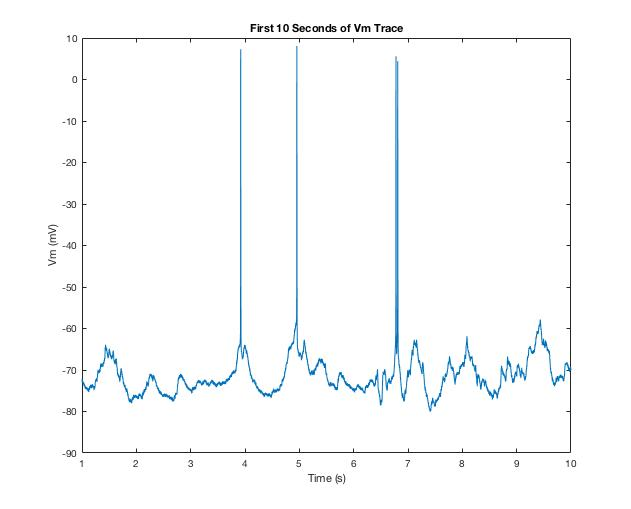
\includegraphics[scale=.5]{vm_sample_trace}


% Problem 2
\hwproblem

List of spike times found in code as variable spikeTimes



% Problem 3
\hwproblem
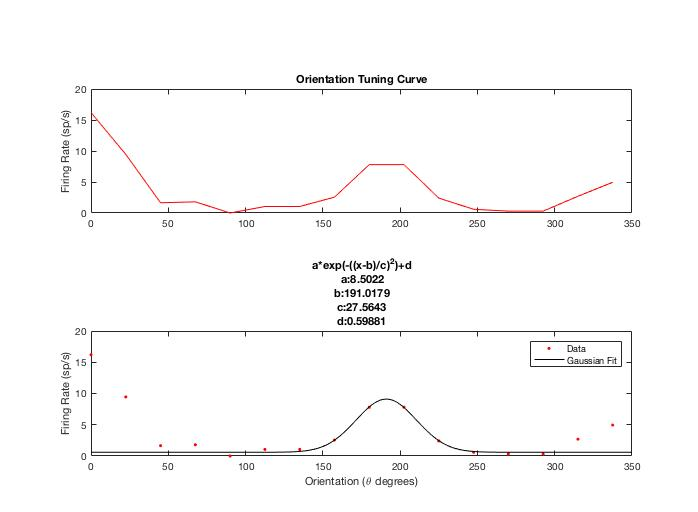
\includegraphics[scale=.75]{tuning_curve}
The preferred orientation angles are ~180 degrees and ~0 degrees. These correspond to motion in opposite directions, with the bar in the same orientation. The 0 degree stimulus has a higher firing rate than the 180 degree stimulus, indicating that maybe the neuron responds to that orientation more strongly in one direction of motion than the other. 

% Problem 4
\hwproblem
Check out the Gaussian in the figure above

% Problem 5
\hwproblem
This was mapping the receptive field of the cell. The receptive field of the cell has an excitatory (green) region and an inhibitory (red) region. For that specific orientation, the one to which the cell is tuned, there is a specific region in visual space mapped to the retina to which this cell responds. The green region is where the cell responds to bright light bars and the red region is where the cell responds to dark bars. This is the same idea as a center-surround RGC receptive field, but it is abstracted to bars of a certain orientation in a certain fragment of the visual field. 






\end{document}